\documentclass[a3paper,xelatex,english]{bxjsarticle}
\usepackage{tikz}%
\usetikzlibrary{arrows.meta,bending,calc,shapes,positioning,shapes.callouts}
\usepackage{ascmac}
\usepackage{fancybox}
\usepackage{amsmath,amssymb}
\usepackage{algorithm}
\usepackage{algpseudocode}
\usepackage{algorithmicx}
\usepackage{paralist}
\usepackage{cases}
\usepackage{url}
\usepackage[unicode,pdftitle={Implementation Notes for entropy estimation based on NIST SP 800-90B non-IID track},setpagesize=false]{hyperref}
\usepackage[open,openlevel=4]{bookmark}
\newcommand\mib[1]{\boldsymbol{#1}}

\usepackage{colortbl}
\usepackage{xcolor}
\usepackage{fancyhdr}
\usepackage[explicit]{titlesec}
\usepackage{xspace}
\usepackage{setspace}

\usetikzlibrary{fit,calc}
%define a marking command
\newcommand*{\tikzmk}[1]{\tikz[remember picture,overlay,] \node (#1) {};\ignorespaces}
%define a boxing command, argument = colour of box
\newcommand{\boxit}[1]{\tikz[remember picture,overlay]{\node[yshift=-10pt,fill=#1,opacity=.25,fit={(A)($(B)+(.90\linewidth,.8\baselineskip)$)}] {};}\ignorespaces}
%define some colours according to algorithm parts (or any other method you like)
\colorlet{hlpink}{red!40}
\colorlet{hlblue}{cyan!60}

% ノードマーク
%%%%%\newcommand*{\tikzmk}[1]{\tikz[remember picture,overlay] \node (#1) {};\ignorespaces}
%%%%%% ボックス描画
%%%%%\newcommand{\boxit}[1]{%
%%%%%  \tikz[remember picture,overlay]{
%%%%%    \node[yshift=3pt,fill=#1,opacity=.25,fit={(A)($(B)+(0.95\linewidth,1.2\baselineskip)$)}] {};
%%%%%  }%
%%%%%  \ignorespaces
%%%%%}
%%%%%% 色定義
%%%%%\colorlet{highlightcolor}{yellow!30}

\usepackage[many]{tcolorbox}
%%%%%%%%%%%%%%%%%%%%%%%%%%%%%%%%%%%%%%%%%%%%%%%%%%%%%%%%%%%%%%%%%%%%%%%%%%%%%%%%
%%%
%%%
%%%
%%%%%%%%%%%%%%%%%%%%%%%%%%%%%%%%%%%%%%%%%%%%%%%%%%%%%%%%%%%%%%%%%%%%%%%%%%%%%%%%
\definecolor{mydarkblue}{RGB}{0,163,243}
\definecolor{mylightblue}{RGB}{191,233,251}
\definecolor{mediumtealblue}{rgb}{0.0, 0.33, 0.71}
\definecolor{BleuDur}{RGB}{27,61,176}
\definecolor{Nigelle}{RGB}{0,133,201}
\definecolor{BleuFaience}{RGB}{105,171,219}
\definecolor{Celeste}{RGB}{0,160,199}
\definecolor{Orseille}{RGB}{243,167,172}
\definecolor{CuisseDeNymph}{RGB}{245,201,193}
\definecolor{Heliotrope}{RGB}{139,92,158}
\definecolor{Pomme}{RGB}{106,186,80}
\definecolor{VertPrintemps}{RGB}{0,152,132}


%%%%%%%%%%%%%%%%%%%%%%%%%%%%%%%%%%%%%%%%%%%%%%%%%%%%%%%%%%%%%%%%%%%%%%%%%%%%%%%%
%%%
%%%
%%%
%%%%%%%%%%%%%%%%%%%%%%%%%%%%%%%%%%%%%%%%%%%%%%%%%%%%%%%%%%%%%%%%%%%%%%%%%%%%%%%%
%\def\chpcolor{blue!45}
\def\chpcolor{mydarkblue}
%\def\chpcolortxt{blue!60}
\def\chpcolortxt{mydarkblue}
\def\sectionfont{\sffamily\LARGE}

%%%%%%%%%%%%%%%%%%%%%%%%%%%%%%%%%%%%%%%%%%%%%%%%%%%%%%%%%%%%%%%%%%%%%%%%%%%%%%%
%%%%%%
%%%%%% 4-th level
%%%%%%
%%%%%%%%%%%%%%%%%%%%%%%%%%%%%%%%%%%%%%%%%%%%%%%%%%%%%%%%%%%%%%%%%%%%%%%%%%%%%%%
\setcounter{secnumdepth}{4}

\setcounter{tocdepth}{4}


\setlength{\textheight}{39cm}
%%%%%%%%%%%%%%%%%%%%%%%%%%%%%%%%%%%%%%%%%%%%%%%%%%%%%%%%%%%%%%%%%%%%%%%%%%%%%%%
%%%%%%
%%%%%%
%%%%%%
%%%%%%%%%%%%%%%%%%%%%%%%%%%%%%%%%%%%%%%%%%%%%%%%%%%%%%%%%%%%%%%%%%%%%%%%%%%%%%%
\makeatletter
%Section:
\def\@sectionstrut{\vrule\@width\z@\@height12.5\p@}
\def\@makesectionhead#1{%
  {\par\vspace{20pt}%
   \parindent 0pt\raggedleft\sectionfont
   \colorbox{\chpcolor}{%
     \parbox[t]{90pt}{\color{white}\@sectionstrut\@depth4.5\p@\hfill
       \ifnum\c@secnumdepth>\z@\thesection\fi}%
   }%
   \begin{minipage}[t]{\dimexpr\textwidth-90pt-2\fboxsep\relax}
   \color{\chpcolortxt}\@sectionstrut\hspace{5pt}#1
   \end{minipage}\par
   \vspace{10pt}%
  }
}
\def\section{\@afterindentfalse\secdef\@section\@ssection}
\def\@section[#1]#2{%
  \ifnum\c@secnumdepth>\m@ne
    \refstepcounter{section}%
    \addcontentsline{toc}{section}{\protect\numberline{\thesection}#1}%
  \else
    \phantomsection
    \addcontentsline{toc}{section}{#1}%
  \fi
  \sectionmark{#1}%
  \if@twocolumn
    \@topnewpage[\@makesectionhead{#2}]%
  \else
    \@makesectionhead{#2}\@afterheading
  \fi
}
\def\@ssection#1{%
  \if@twocolumn
    \@topnewpage[\@makesectionhead{#1}]%
  \else
    \@makesectionhead{#1}\@afterheading
  \fi
}
\makeatother
%%%%%%%%%%%%%%%%%%%%%%%%%%%%%%%%%%%%%%%%%%%%%%%%%%%%%%%%%%%%%%%%%%%%%%%%%%%%%%%%
%%%
%%%
%%%
%%%%%%%%%%%%%%%%%%%%%%%%%%%%%%%%%%%%%%%%%%%%%%%%%%%%%%%%%%%%%%%%%%%%%%%%%%%%%%%%
\newsavebox\mybox
\newlength\secnumwd

%\definecolor{mydarkblue}{RGB}{0,163,243}
%\definecolor{mylightblue}{RGB}{191,233,251}

\titleformat{\section}
  {\normalfont\Large\sffamily\color{mydarkblue}}
  {}
  {-5em}
  {%
    \savebox\mybox{\normalfont\Large\sffamily\color{mydarkblue}\bfseries\thesection}%
    \settowidth\secnumwd{\usebox\mybox}%    
    \parbox[t]{\secnumwd}{{\bfseries\thesection}}\hspace{1em}%
    \parbox[t]{\dimexpr\textwidth+5em-\secnumwd-1em\relax}{#1}%
  }
  [\vskip-1.75ex\hskip-5em{\color{gray!60}\titlerule[2pt]}]
\titleformat{name=\section,numberless}
  {\normalfont\Large\sffamily\color{mydarkblue}}
  {}
  {-5em}
  {#1}
  [\vskip-1.75ex\hskip-5em{\color{gray!60}\titlerule[2pt]}]

\newcommand\FrameBoxL[1]{%
  \fcolorbox{mylightblue}{mydarkblue}{\makebox[3cm][l]{\textcolor{white}{\bfseries#1}}}%
}
\newcommand\FrameBoxR[1]{%
  \fcolorbox{mylightblue}{mydarkblue}{\makebox[3cm][r]{\textcolor{white}{\bfseries#1}}}%
}

\pagestyle{fancy}
\fancyheadoffset[EL]{\dimexpr1in+\evensidemargin+\hoffset\relax}
\fancyheadoffset[OR]{\dimexpr\paperwidth-\oddsidemargin-1in-\textwidth-\hoffset\relax}
\fancyhf{}
\renewcommand\headrulewidth{0pt}
\fancyhead[OR]{\FrameBoxL{\thepage}}
\fancyhead[EL]{\FrameBoxR{\thepage}}
%%%%%%%%%%%%%%%%%%%%%%%%%%%%%%%%%%%%%%%%%%%%%%%%%%%%%%%%%%%%%%%%%%%%%%%%%%%%%%%%
%%%
%%% argmax
%%%
%%%%%%%%%%%%%%%%%%%%%%%%%%%%%%%%%%%%%%%%%%%%%%%%%%%%%%%%%%%%%%%%%%%%%%%%%%%%%%%%
\newcommand{\argmax}{\mathop{\textrm{arg~max}}\limits}
%%%%%%%%%%%%%%%%%%%%%%%%%%%%%%%%%%%%%%%%%%%%%%%%%%%%%%%%%%%%%%%%%%%%%%%%%%%%%%%%
%%%
%%% vertical equal
%%%
%%%%%%%%%%%%%%%%%%%%%%%%%%%%%%%%%%%%%%%%%%%%%%%%%%%%%%%%%%%%%%%%%%%%%%%%%%%%%%%%
\newcommand\rotateequal[1]{%
  \ifmmode
    \underset{#1}{\rotatebox{90}{$=$}}%
  \fi
}
%%%%%%%%%%%%%%%%%%%%%%%%%%%%%%%%%%%%%%%%%%%%%%%%%%%%%%%%%%%%%%%%%%%%%%%%%%%%%%%%
%%%
%%%
%%%
%%%%%%%%%%%%%%%%%%%%%%%%%%%%%%%%%%%%%%%%%%%%%%%%%%%%%%%%%%%%%%%%%%%%%%%%%%%%%%%%
\algnewcommand{\algorithmicgoto}{\textbf{go to}}%
\algnewcommand{\Goto}{\algorithmicgoto\xspace}%
\algnewcommand{\Label}{\State\unskip}
\algnewcommand{\Downto}{\textbf{ downto }}


\renewcommand{\algorithmicrequire}{\textbf{Input:}}  % Use Input in the format of Algorithm  
\renewcommand{\algorithmicensure}{\textbf{Output:}} % Use Output in the format of Algorithm  

\algdef{SE}[PROCEDURE]{Procedure}{EndProcedure}%
   [2]{\algorithmicprocedure\ \textproc{#1}\ifthenelse{\equal{#2}{}}{}{(#2)}}%
   {\algorithmicend\ \algorithmicprocedure}%
\algdef{SE}[FUNCTION]{Function}{EndFunction}%
   [2]{\algorithmicfunction\ \textproc{#1}\ifthenelse{\equal{#2}{}}{}{(#2)}}%
   {\algorithmicend\ \algorithmicfunction}%


%%%%%%%%%%%%%%%%%%%%%%%%%%%%%%%%%%%%%%%%%%%%%%%%%%%%%%%%%%%%%%%%%%%%%%%%%%%%%%%%
%%%
%%%
%%%
%%%%%%%%%%%%%%%%%%%%%%%%%%%%%%%%%%%%%%%%%%%%%%%%%%%%%%%%%%%%%%%%%%%%%%%%%%%%%%%%
\definecolor{myblue}{RGB}{0,163,243}

\newtcolorbox[auto counter,number within=section]{mytheorem}[1][]{
  enhanced jigsaw,colback=white,colframe=myblue,coltitle=myblue,
  fonttitle=\bfseries\sffamily,
  sharp corners,
  detach title,
  leftrule=22mm,
  underlay unbroken and first={\node[below,text=white,font=\sffamily\bfseries,align=center]
    at ([xshift=-11mm,yshift=-1mm]interior.north west) {THEOREM\\\thetcbcounter};},
  breakable,pad at break=1mm,
  #1,
  code={\ifdefempty{\tcbtitletext}{}{\tcbset{before upper={\tcbtitle\par\medskip}}}},
}

%%%\usepackage{titlesec}
%%%%%%\usepackage{lipsum}
%%%\usepackage{tikz}\usetikzlibrary{shapes.misc}
%%%\newcommand\titlebar{%
%%%\tikz[baseline,trim left=3.1cm,trim right=3cm] {
%%%    \fill [cyan!25] (2.5cm,-1ex) rectangle (\textwidth+3.1cm,2.5ex);
%%%    \node [
%%%        fill=cyan!60!white,
%%%        anchor= base east,
%%%        %rounded rectangle,
%%%        rectangle,
%%%        minimum height=3.5ex] at (3cm,0) {
%%%        \textbf{\thesection.}
%%%    };
%%%}%
%%%}
%%%\titleformat{\section}{\large}{\titlebar}{0.1cm}{}
%%%\renewcommand*{\thesection}{\arabic{section}}

%%%\usepackage{xcolor}
%%%
%%%\setcounter{section}{1} % just to emulate a chapter has started
%%%
%%%\renewcommand*{\othersectionlevelsformat}[1]{%
%%%  \makebox[0pt][r]{%
%%%    \fcolorbox{cyan!60!white}{cyan!60!white}{\color{white}\csname the#1\endcsname}%
%%%    \enskip
%%%  }
%%%}


\renewcommand{\figurename}{Figure }
\renewcommand{\tablename}{Table }
\renewcommand{\refname}{References}
\renewcommand*{\thesection}{\arabic{section}}
\author{Gen'ya SAKURAI}
\title{Implementation Notes for \\entropy estimation based on NIST SP 800-90B non-IID track}
\date{\today}
\begin{document}
\maketitle
%%%%%%%%%%%%%%%%%%%%%%%%%%%%%%%%%%%%%%%%%%%%%%%%%%%%%%%%%%%%%%%%%%%
%%%%%
%%%%%
%%%%%
%%%%%%%%%%%%%%%%%%%%%%%%%%%%%%%%%%%%%%%%%%%%%%%%%%%%%%%%%%%%%%%%%%%
\section{Implementation notes for numerical computation of entropy estimates}
\renewcommand{\arraystretch}{1.4}
%%%%%%%%%%%%%%%%%%%%%%%%%%%%%%%%%%%%%%%%%%%%%%%%%%%%%%%%%%%%%%%%%%%
%%%%%
%%%%%
%%%%%
%%%%%%%%%%%%%%%%%%%%%%%%%%%%%%%%%%%%%%%%%%%%%%%%%%%%%%%%%%%%%%%%%%%
\subsection{Notes for the Markov estimate}
In this section, we follow the convention using a column vector of probabilities $\mib{P}$ and a left stochastic matrix $\mib{T}$.
\begin{align}
\mib{P} 
\equiv 
& 
\begin{bmatrix}
p_{0} \\
p_{1} \\
\end{bmatrix} 
\\
%%%%%
%%%%%
%%%%%
\mib{T} 
\equiv 
& 
\begin{bmatrix}
t_{0,0} & t_{0,1} \\
t_{1,0} & t_{1,1}
\end{bmatrix}
\end{align}
Note here that 6.3.3 of NIST SP 800-90B\cite{SP80090B} uses the convention of a row vector of probabilities and a right stochastic matrix.  So the transition matrix components $t_{i,j}$ in this section will be interpreted as $P_{j,i}$ in 6.3.3 of NIST SP 800-90B\cite{SP80090B}.


Considering a sequence of binary-valued samples of length $\lambda$, there are following four possible combinations of the first sample value and the last sample value:\begin{enumerate}[a)]
	\item 0 $\to$ 0
	\item 0 $\to$ 1
	\item 1 $\to$ 0
	\item 1 $\to$ 1
\end{enumerate}

For each combination, the probability of occurrence of the most likely sequence is expressed by the following equation, by using the parameters $\mu$ and $\nu$:
\begin{enumerate}[a)]
	%%%%%
	%%%%% a)
	%%%%%
	\item 
	\begin{align}
		f_{a}(\mib{T}, \mu, \nu) & \equiv p_{0} t_{00}^{\nu} t_{11}^{\lambda - 1 - 2\mu - \nu} t_{01}^{\mu} t_{10}^{\mu} 
	\end{align}
	\begin{align}
	\begin{cases}
		0 \leq 2 \mu < \lambda - 1 & \\
		0 \leq \nu \leq \lambda - 1 & \\
		0 \leq \lambda - 1 - 2\mu - \nu \leq \lambda - 1
	\end{cases}
	\label{eq:fa}
	\end{align}
	%%%%%
	%%%%% b)
	%%%%%
	\item 
	\begin{align}
		f_{b}(\mib{T}, \mu, \nu) & \equiv p_{0} t_{00}^{\nu} t_{11}^{\lambda - 2 - 2\mu - \nu} t_{01}^{\mu} t_{10}^{\mu + 1} 
	\end{align}
	\begin{align}
	\begin{cases}
		0 \leq 2 \mu < \lambda - 1 & \\
		0 \leq \nu < \lambda - 1 & \\
		0 \leq \lambda - 2 - 2\mu - \nu \leq \lambda - 2
	\end{cases}
	\label{eq:fb}
	\end{align}
	%%%%%
	%%%%% c)
	%%%%%
	\item 
	\begin{align}
		f_{c}(\mib{T}, \mu, \nu) & \equiv p_{1} t_{00}^{\nu} t_{11}^{\lambda - 2 - 2\mu - \nu} t_{01}^{\mu + 1} t_{10}^{\mu} 
	\end{align}
	\begin{align}
	\begin{cases}
		0 \leq 2 \mu < \lambda - 1 & \\
		0 \leq \nu < \lambda - 1 & \\
		0 \leq \lambda - 2 - 2\mu - \nu \leq \lambda - 2
	\end{cases}
	\label{eq:fc}
	\end{align}
	%%%%%
	%%%%% d)
	%%%%%
	\item 
	\begin{align}
		f_{d}(\mib{T}, \mu, \nu) & \equiv p_{1} t_{00}^{\nu} t_{11}^{\lambda - 1 - 2\mu - \nu} t_{01}^{\mu} t_{10}^{\mu} 
	\end{align}
	\begin{align}
	\begin{cases}
		0 \leq 2 \mu < \lambda - 1 & \\
		0 \leq \nu \leq \lambda - 1 & \\
		0 \leq \lambda - 1 - 2\mu - \nu \leq \lambda - 1
	\end{cases}
	\label{eq:fd}
	\end{align}
\end{enumerate}

If we denote $\kappa$ as the exponent of $t_{11}$, then the possible values of $\mu, \nu$, and $\kappa$ are expressed as integer coordinates in the approximately triangular region (to be precise, truncated triangle) shown in Figure \ref{fig:parameterplane}.
\begin{figure}[htbp]
\centering

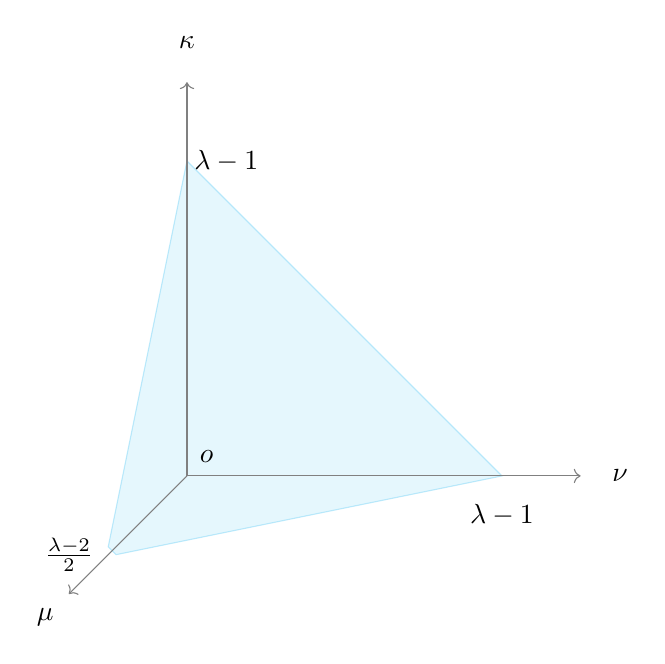
\begin{tikzpicture}
	\filldraw[fill=cyan!20, draw=cyan!50, opacity=0.5] (-0.9, -1) -- (4, 0) -- (0, 4) -- (-1, -0.9) -- (-0.9, -1);
	\draw[->,gray] ( 0, 0) -- (5, 0);
	\draw[->,gray] ( 0, 0) -- (0, 5);
	\draw[->,gray] ( 0, 0) -- (-1.5, -1.5);
	\draw (5.5, 0) node {$\nu$} ;
	\draw (-1.8, -1.8) node {$\mu$} ;
	\draw (0, 5.5) node {$\kappa$} ;
	%%%%%
	\draw ( 0.25, 0.25) node {$o$} ;
	\draw ( 4, -0.5) node {$\lambda - 1$} ;
	\draw ( 0.5,  4) node {$\lambda - 1$} ;
	\draw (-1.5, -1) node {$\frac{\lambda - 2}{2}$} ;
\end{tikzpicture}

\caption{Parameter plane of the exponents $\kappa$, $\mu$, $\nu$}
\label{fig:parameterplane}
\end{figure}

In order to calculate the extrema of $f_{a}, f_{b}, f_{c}$, and $f_{d}$, assuming that $\mu$, and $\nu$ are continuous variables, we first consider the partial derivatives of $f_{a}(\mib{T}, \mu, \nu)$ with respect to $\mu$, and $\nu$.

\begin{align}
	\frac{\partial }{\partial \mu} f_{a}(\mib{T}, \mu, \nu) 
	&= 
	(-2 \ln t_{11} + \ln t_{01} + \ln t_{10}) f_{a}(\mib{T}, \mu, \nu) 
	\nonumber \\
	&= 
	\ln \frac{t_{01} t_{10}}{t_{11}^{2}} 
	f_{a}(\mib{T}, \mu, \nu) 
	\label{eq:nondiagonalproduct}
	\\
	%%%%%
	\frac{\partial }{\partial \nu} f_{a}(\mib{T}, \mu, \nu) 
	&= 
	(\ln t_{00} - \ln t_{11}) f_{a}(\mib{T}, \mu, \nu) 
	\nonumber \\
	&= 
	\ln \frac{t_{00}}{t_{11}} 
	f_{a}(\mib{T}, \mu, \nu) 
	\label{eq:diagonal}
\end{align}

%The partial derivatives of $f_{b}, f_{c}$, and $f_{d}$ with respect to $\mu$ and $\nu$ are obtained by taking permutation of $a$ with respecto to $b$, $c$, and $d$ in eq. (\ref{eq:nondiagonalproduct}) and eq.(\ref{eq:diagonal}), respectively.

Taking into accout eqs. (\ref{eq:nondiagonalproduct}) and (\ref{eq:diagonal}), and the property that the value $f_{a}(\mib{T}, \mu, \nu)$ is non-negative, 
a rough phase diagram will be obtained as shown in Figure \ref{fig:phasediagram}, by taking the horizontal axis as $\ln \frac{t_{00}}{t_{11}}$, and the vertical axis as $\tfrac{1}{2}\ln \frac{t_{01} t_{10}}{t_{11}^{2}}$.

\begin{figure}[htbp]
\centering

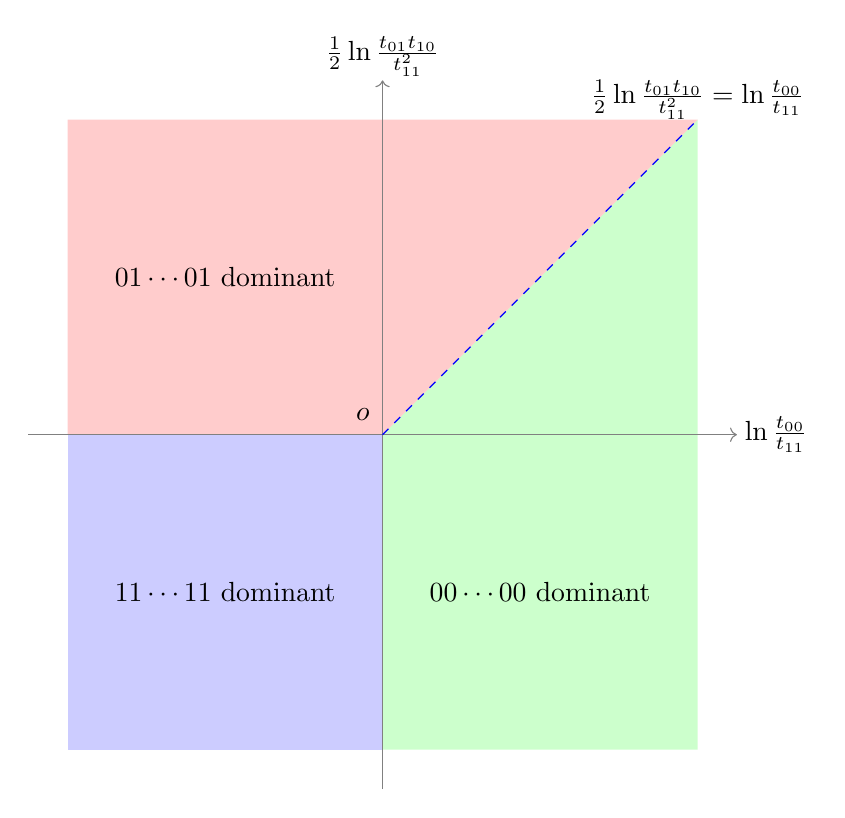
\begin{tikzpicture}
	\fill[green!20] (0, 0) -- (4,4) -- (4, -4) -- (0, -4);
	\fill[red!20] (0, 0) -- (4, 4) -- (-4,4) -- (-4, 0);
	\fill[blue!20] (0, 0) -- (0, -4) -- (-4,-4) -- (-4, 0);
	\draw[->,gray] (-4.5, 0) -- (4.5, 0);
	\draw[->,gray] ( 0,-4.5) -- (0, 4.5);
	\draw (-0.25, 0.25) node {$o$} ;
	\draw (5, 0) node {$\ln \frac{t_{00}}{t_{11}}$} ;
	\draw (0, 4.8) node {$\tfrac{1}{2} \ln \frac{t_{01} t_{10}}{t_{11}^{2}}$} ;
	\draw[blue,dashed] (0, 0) -- (4, 4);
	\draw (4, 4.25) node {$\tfrac{1}{2} \ln \frac{t_{01} t_{10}}{t_{11}^{2}} = \ln \frac{t_{00}}{t_{11}}$} ;
	%%%%%
	\draw ( 2, -2) node {$00 \cdots 00$ dominant} ;
	\draw (-2,  2) node {$01 \cdots 01$ dominant} ;
	\draw (-2, -2) node {$11 \cdots 11$ dominant} ;
\end{tikzpicture}

\caption{Phase diagram of most likely sequence based on $f_{a}(\mib{T}, \mu, \nu)$ with respect to components of stochastic matrix $\mib{T}$}
\label{fig:phasediagram}
\end{figure}

First, if we consider the third quadrant, for example, the conditional probability $t_{11}$ is greater than or equal to $t_{00}$ and $\sqrt{t_{01}t_{10}}$, then the sequence $11 \cdots 11$ will be dominant.

Next, for the other quadrants, let us consider whether $00 \cdots 00$ or $01 \cdots 01$ is the dominant sequence. 
In particular, for the first quadrant, since right hand sides of eqs. (\ref{eq:nondiagonalproduct}) and (\ref{eq:diagonal}) are positive, let us examine whether $00 \cdots 00$ or $0101 \cdots 0101$ is the dominant sequence. 
Since at least $11 \cdots 11$ is not a dominant sequence, we can limit the discussion with $\kappa =$ 0, 1, the parameter region of possible values of $\mu$ and $\nu$ is restricted to a line segment in Figure \ref{fig:parameterplane}. 
In this case, the total differentiation of $f_{a}$ is then expressed by the following equation:
\begin{align}
\Delta f_{a} 
&= 
\left( 
\frac{\partial f_{a}}{\partial \mu} 
+ 
\frac{\partial f_{a}}{\partial \nu} 
\frac{{\mathrm d} \nu}{{\mathrm d} \mu}
\right) 
\Delta \mu 
\nonumber 
\\
&= 
\left(
\ln \frac{t_{01}t_{10}}{t_{00}^{2}}
\right)
\Delta \mu
	\label{expression:totaldiff}
\end{align}

From this equation, if RHS of eq. (\ref{expression:totaldiff}) is positive, $f_{a}$ increases with respect to $\mu$ and $01 \cdots 01$ becomes the dominant sequence, and conversely, if RHS of eq. (\ref{expression:totaldiff}) is negative, $00 \cdots 00$ becomes the dominant sequence.
This will be determined by the following coefficient:

\begin{align}
	\ln \frac{t_{01}t_{10}}{t_{00}^{2}} 
	&= 
	\ln \frac{t_{01}t_{10}}{t_{11}^{2}} - 2 \ln \frac{t_{00}}{t_{11}}
	\label{expression:separationline}
\end{align}
Figure \ref{fig:phasediagram} shows a dashed diagonal straight line in the first quadrant, on which the RHS of eq. (\ref{expression:separationline}) is zero.  
In other words, in the region above this line, $01 \cdots 01$ is the dominant sequence, and $00 \cdots 00$ is the dominant sequence in the region below the line. 


From the above, we have to consider the following three dominant sequences:
\begin{enumerate}[i)]
	\item $00 \cdots 00$ dominant 
	\item $01 \cdots 01$ dominant 
	\item $11 \cdots 11$ dominant 
\end{enumerate}
For each combination of $f_a, f_b, f_c$, $f_d$, and above three dominant sequences i), ii), and iii), 
the following expressions are obtained giving the maximum probability with respect to $\mu$ and $\nu$:

\begin{enumerate}[{a)}-i)]
	\item $00 \cdots 00$ dominant 
	\begin{align}
	\max_{\mu, \nu}(f_{a}(\mib{T}, \mu, \nu)) = p_{0} t_{00}^{\lambda - 1}
	\end{align}
	\item $01 \cdots 01$ dominant 
	\begin{align}
	\max_{\mu, \nu}(f_{a}(\mib{T}, \mu, \nu)) = & p_{0} t_{00} t_{01}^{(\lambda - 2) / 2} t_{10}^{(\lambda - 2) / 2}, {\textrm{or}} \\
	\max_{\mu, \nu}(f_{a}(\mib{T}, \mu, \nu)) = & p_{0} t_{11} t_{01}^{(\lambda - 2) / 2} t_{10}^{(\lambda - 2) / 2}
	\end{align}
	\item $11 \cdots 11$ dominant 
	\begin{align}
	\max_{\mu, \nu}(f_{a}(\mib{T}, \mu, \nu)) = p_{0} t_{11}^{\lambda - 3} t_{01} t_{10} \label{expression:neg1}
	\end{align}
\end{enumerate}

\begin{enumerate}[{b)}-i)]
	\item $00 \cdots 00$ dominant 
	\begin{align}
	\max_{\mu, \nu}(f_{b}(\mib{T}, \mu, \nu)) = p_{0} t_{00}^{\lambda - 2} t_{10}
	 \label{expression:nonneg1}
	\end{align}
	\item $01 \cdots 01$ dominant 
	\begin{align}
	\max_{\mu, \nu}(f_{b}(\mib{T}, \mu, \nu)) = p_{0} t_{01}^{(\lambda - 2) / 2} t_{10}^{\lambda / 2}
	\end{align}
	\item $11 \cdots 11$ dominant 
	\begin{align}
	\max_{\mu, \nu}(f_{b}(\mib{T}, \mu, \nu)) = p_{0} t_{11}^{\lambda - 2} t_{10} \label{expression:neg2}
	\end{align}
\end{enumerate}

\begin{enumerate}[{c)}-i)]
	\item $00 \cdots 00$ dominant 
	\begin{align}
	\max_{\mu, \nu}(f_{c}(\mib{T}, \mu, \nu)) = p_{1} t_{00}^{\lambda - 2} t_{01} \label{expression:neg3}
	\end{align}
	\item $01 \cdots 01$ dominant 
	\begin{align}
	\max_{\mu, \nu}(f_{c}(\mib{T}, \mu, \nu)) = p_{1} t_{01}^{\lambda / 2} t_{10}^{(\lambda - 2) / 2}
	\end{align}
	\item $11 \cdots 11$ dominant 
	\begin{align}
	\max_{\mu, \nu}(f_{c}(\mib{T}, \mu, \nu)) = p_{1} t_{11}^{\lambda - 2} t_{01}
	\end{align}
\end{enumerate}

\begin{enumerate}[{d)}-i)]
	\item $00 \cdots 00$ dominant 
	\begin{align}
	\max_{\mu, \nu}(f_{d}(\mib{T}, \mu, \nu)) = p_{1} t_{00}^{\lambda - 3} t_{01} t_{10} \label{expression:neg4}
	\end{align}
	\item $01 \cdots 01$ dominant 
	\begin{align}
	\max_{\mu, \nu}(f_{d}(\mib{T}, \mu, \nu)) = & p_{1} t_{00} t_{01}^{(\lambda - 2) / 2} t_{10}^{(\lambda - 2) / 2}, {\textrm{or}} \\
	\max_{\mu, \nu}(f_{d}(\mib{T}, \mu, \nu)) = & p_{1} t_{11} t_{01}^{(\lambda - 2) / 2} t_{10}^{(\lambda - 2) / 2}
	\end{align}
	\item $11 \cdots 11$ dominant 
	\begin{align}
	\max_{\mu, \nu}(f_{d}(\mib{T}, \mu, \nu)) = p_{1} t_{11}^{\lambda - 1}
	\end{align}
\end{enumerate}
Note here that we considered the property that $\lambda$ is even in the above expressions.
Also note that all bounary conditions are considered in the above calculation, combination of first sample values and last sample values.


From the above, we have to compare 14 expressions listed in Table \ref{tab:ListProbabilitiesMostLikelySequences}.

\begin{table}[htbp]
\caption{Probabilities of the most or second most likely sequences of length $\lambda$}
\label{tab:ListProbabilitiesMostLikelySequences}
%\begin{center}
\makebox[\textwidth][c]{
\begin{tabular}{|r|l|c|c|l|}
\hline
\rowcolor{mylightblue} %%
No. & Sequence & Probability & $-\log_{2} ({\textrm{Probability}}) / \lambda$ & Notes\\
\hline 
1 & $0000 \cdots 0000$ & $p_{0} \times t_{00}^{\lambda - 1}$ & $-\left[ \frac{\lambda - 1}{\lambda} \log_{2} t_{00} + \frac{1}{\lambda} \log_{2} p_{0} \right]$ & $^{\textrm{\,a}}$, $^{\textrm{\,b}}$\\
\hline
2 & $0101 \cdots 0101001010 \cdots 1010$ & $p_{0} \times t_{00} \times t_{01}^{(\lambda - 2) / 2} \times t_{10}^{(\lambda - 2) / 2}$ & $-\left[ \frac{\lambda - 2}{2\lambda} \log_{2} \left( t_{01} t_{10} \right) + \frac{1}{\lambda} \log_{2} \left( p_{0} \times t_{00} \right) \right]$ & \quad $^{\textrm{\,\,b}}$ \\
\hline
3 & $0101 \cdots 0101101010 \cdots 1010$ & $p_{0} \times t_{11} \times t_{01}^{(\lambda - 2) / 2} \times t_{10}^{(\lambda - 2) / 2}$ & $-\left[ \frac{\lambda - 2}{2\lambda} \log_{2} \left( t_{01} t_{10} \right) + \frac{1}{\lambda} \log_{2} \left( p_{0} \times t_{11} \right) \right]$ &  \\
\hline 
4 & $0111 \cdots 1110$ & $p_{0} \times t_{11}^{\lambda - 3} \times t_{01} \times t_{10}$ & $-\left[ \frac{\lambda - 3}{\lambda} \log_{2} t_{11}+ \frac{1}{\lambda} \log_{2} \left( p_{0} \times t_{01} \times t_{10} \right)\right]$ &  \\
\hline 
5 & $0000 \cdots 0001$ & $p_{0} \times t_{00}^{\lambda - 2} \times t_{10}$ & $-\left[ \frac{\lambda - 2}{\lambda} \log_{2} t_{00}+ \frac{1}{\lambda} \log_{2} \left( p_{0} \times t_{10} \right)\right]$ &  \\
\hline 
6 & $0101 \cdots 0101$ & $p_{0} \times t_{01}^{(\lambda - 2) / 2} \times t_{10}^{\lambda / 2}$ & $-\left[ \frac{\lambda - 2}{2\lambda} \log_{2} \left( t_{01} t_{10} \right) + \frac{1}{\lambda} \log_{2} \left( p_{0} \times t_{10} \right) \right]$ & $^{\textrm{\,a}}$, $^{\textrm{\,b}}$ \\
\hline 
7 & $0111 \cdots 1111$ & $p_{0} \times t_{11}^{\lambda - 2} \times t_{10}$ & $-\left[ \frac{\lambda - 2}{\lambda} \log_{2} t_{11}+ \frac{1}{\lambda} \log_{2} \left( p_{0} \times t_{10} \right)\right]$ & $^{\textrm{\,a}}$, \quad $^{\textrm{\,c}}$\\
\hline 
8 & $1000 \cdots 0000$ & $p_{1} \times t_{00}^{\lambda - 2} \times t_{01}$ & $-\left[ \frac{\lambda - 2}{\lambda} \log_{2} t_{00}+ \frac{1}{\lambda} \log_{2} \left( p_{1} \times t_{01} \right)\right]$ & $^{\textrm{\,a}}$, $^{\textrm{\,b}}$ \\
\hline 
9 & $1010 \cdots 1010$ & $p_{1} \times t_{01}^{\lambda / 2} \times t_{10}^{(\lambda - 2) / 2}$ & $-\left[ \frac{\lambda - 2}{2\lambda} \log_{2} \left( t_{01} t_{10} \right) + \frac{1}{\lambda} \log_{2} \left( p_{1} \times t_{01} \right) \right]$ & $^{\textrm{\,a}}$, $^{\textrm{\,b}}$ \\
\hline 
10 & $1111 \cdots 1110$ & $p_{1} \times t_{11}^{\lambda - 2} \times t_{01}$ & $-\left[ \frac{\lambda - 2}{\lambda} \log_{2} t_{11}+ \frac{1}{\lambda} \log_{2} \left( p_{1} \times t_{01} \right)\right]$ &  \\
\hline 
11 & $1000 \cdots 0001$ & $p_{1} \times t_{00}^{\lambda - 3} \times t_{01} \times t_{10}$ & $-\left[ \frac{\lambda - 3}{\lambda} \log_{2} t_{00} + \frac{1}{\lambda} \log_{2} \left( p_{1} \times t_{01} \times t_{10} \right) \right]$ &  \\
\hline
12 & $1010 \cdots 1010100101 \cdots 0101$ & $p_{1} \times t_{00} \times t_{01}^{(\lambda - 2) / 2} \times t_{10}^{(\lambda - 2) / 2}$ & $-\left[ \frac{\lambda - 2}{2\lambda} \log_{2} \left( t_{01} t_{10} \right) + \frac{1}{\lambda} \log_{2} \left( p_{1} \times t_{00} \right) \right]$ &  \\
\hline
13 & $1010 \cdots 1010110101 \cdots 0101$ & $p_{1} \times t_{11} \times t_{01}^{(\lambda - 2) / 2} \times t_{10}^{(\lambda - 2) / 2}$ & $-\left[ \frac{\lambda - 2}{2\lambda} \log_{2} \left( t_{01} t_{10} \right) + \frac{1}{\lambda} \log_{2} \left( p_{1} \times t_{11} \right) \right]$ & \qquad $^{\textrm{\,c}}$ \\
\hline 
14 & $1111 \cdots 1111$ & $p_{1} \times t_{11}^{\lambda - 1}$ & $-\left[ \frac{\lambda - 1}{\lambda} \log_{2} t_{11} + \frac{1}{\lambda} \log_{2} p_{1} \right]$ & $^{\textrm{\,a}}$, $^{\textrm{\,b}}$ \\
\hline 
\hline 
\multicolumn{5}{|l|}{$^{\textrm{\,a}}$\quad Included in 6.3.3 of NIST SP 800-90B\cite{SP80090B}.} \\ 
\multicolumn{5}{|l|}{$^{\textrm{\,b}}$\quad Explicitly included in paragraph 516 of AIS 20/31 Version 2.35 - DRAFT \cite{AIS31draft2022}, by using the relation $m \equiv \lambda - 1$.} \\ 
\multicolumn{5}{|p{17cm}|}{$^{\textrm{\,c}}$\quad Implicitly included in paragraph 516 of AIS 20/31 Version 2.35 - DRAFT \cite{AIS31draft2022}, by using the relation $m \equiv \lambda - 1$ and by relabeling the state space $\Omega$ = \{0, 1\}.} \\ 
\hline 
\end{tabular}
}
%\end{center}
\end{table}

\clearpage
%%%%%%%%%%%%%%%%%%%%%%%%%%%%%%%%%%%%%%%%%%%%%%%%%%%%%%%%%%%%%%%%%%%
%%%%%
%%%%%
%%%%%
%%%%%%%%%%%%%%%%%%%%%%%%%%%%%%%%%%%%%%%%%%%%%%%%%%%%%%%%%%%%%%%%%%%
\subsection{Notes for the collision estimate}
In this section, we try to rewrite the following equation using elementary functions:
\begin{align}
F(1/z) = \Gamma(3,z)z^{-3}\exp(z) 
\label{eq:Fin632}
\end{align}
In NIST SP 800-90B\cite{SP80090B}, it is documented to evaluate incomplete gamma function using continued fraction.
However, we try to obtain simpler expression using known properties of incomplete gamma function without using continued fraction.

First we try to use the following equations (see 8.4.8 and 8.4.11 in \cite{MathHandbook}).
\begin{align}
\Gamma(n + 1, z) &= n!\exp(-z) e_{n}(z), \\
e_{n}(z) &= \sum_{k = 0}^{n}\frac{z^{k}}{k!}
\end{align}
With these two equations, $F(1/z)$ can be rewritten to as follows:
\begin{align}
F(1/z) &= \Gamma(3,z)z^{-3}\exp(z) \nonumber \\
&= 2!\exp(-z) e_{2}(z) z^{-3} \exp(z) \nonumber \\
&= 2 z^{-3} e_{2}(z) \nonumber \\
&= 2 z^{-3} \sum_{k = 0}^{2}\frac{z^{k}}{k!} \nonumber \\
&= 2 z^{-3} \left( 1 + z + \frac{z^{2}}{2} \right) \nonumber \\
&= z^{-1} \left( 2z^{-2} + 2z^{-1} + 1 \right) 
\label{eq:rewFin632}
\end{align}
By replacing the argument $1/z$ with $q$, the following expression can be obtained:
\begin{align}
F(q) &= q \left( 2q^{2} + 2q + 1 \right) \label{eq:rewFin632final}
\end{align}
From this expression, the range of $F(q)$ is $[0, \frac{5}{4}]$, with respect to the domain $q \in [0, 0.5]$.

If we denote $g(p)$ as the right hand side (RHS) of equation to be solved, in step 7 of 6.3.2 of NIST SP 800-90B\cite{SP80090B}, $g(p)$ can be rewritten by using Eq.(\ref{eq:rewFin632final}).
\begin{align}
g(p) & \equiv  p q^{-2} \left[ 1 + \frac{1}{2}(p^{-1} - q^{-1}) \right]F(q) - p q^{-1} \frac{1}{2}(p^{-1} - q^{-1}) \nonumber \\
&= p q^{-2} \left[ 1 + \frac{1}{2}(p^{-1} - q^{-1}) \right]q \left( 2q^{2} + 2q + 1 \right) - p q^{-1} \frac{1}{2}(p^{-1} - q^{-1}) \nonumber \\
&= p q^{-1} \left[ 1 + \frac{1}{2}(p^{-1} - q^{-1}) \right]  \left( 2q^{2} + 2q + 1 \right) - p q^{-1} \frac{1}{2}(p^{-1} - q^{-1}) \nonumber \\
&= p q^{-1} \left[ 1 + \frac{1}{2}(p^{-1} - q^{-1}) \right] - p q^{-1} \frac{1}{2}(p^{-1} - q^{-1}) \nonumber \\
&+ p q^{-1} \left[ 1 + \frac{1}{2}(p^{-1} - q^{-1}) \right] \left( 2q^{2} + 2q \right) \nonumber \\
&= p q^{-1} 
 + 2 p \left[ 1 + \frac{1}{2}(p^{-1} - q^{-1}) \right] \left( q + 1 \right) \nonumber \\
&= p q^{-1} 
 + 2 p \left[ (q + 1) + \frac{1}{2}p^{-1}(q + 1) - \frac{1}{2}(1 + q^{-1}) \right] \nonumber \\
&= p q^{-1} 
 + p \left[ 2(q + 1) + p^{-1}(q + 1) - (1 + q^{-1}) \right] \nonumber \\
&= p \left[ 2(q + 1) + p^{-1}(q + 1) - 1 \right] \nonumber \\
&= p \left[ 2q + 1 + p^{-1}(q + 1) \right] \nonumber \\
&= \left( 2pq + p + q + 1 \right) \nonumber \\
&= \left( 2pq + 2 \right) \nonumber \\
&= 2( pq + 1) \nonumber \\
&= 2 \left[ p(1 - p) + 1 \right] \nonumber \\
&= 2 \left[ -\left(p - \frac{1}{2}\right)^{2} + \frac{5}{4} \right] \label{eq:rhs632}
\end{align}

Figure \ref{fig:rhs632} shows Eq.(\ref{eq:rhs632}) graphically.
\begin{figure}[htbp]
\centering

\begin{tikzpicture}[scale=3]
\draw[very thin,color=gray,loosely dotted] (-0.1,-0.1) grid (1.1,3.1);
\draw[->] (-0.2,0) -- (1.4,0) node[right] {$p$};
\draw[->] (0,-0.2) -- (0,3.4) node[above] {\shortstack{RHS of equation in step 7 \\$\equiv g(p)$}};
\draw[domain=0.5:1, smooth, variable=\x, color=blue] plot (\x,{2*(\x*(1-\x)+1)}) node[above right, xshift = 10pt, yshift = 10pt] {$g(p) = 2 \left[ p (1 - p) + 1 \right] $};
\draw[gray,dotted] (  0.5,2.5) -- ( 0.0,2.5);
\draw[gray,dotted] (  0.5,2.5) -- ( 0.5,0);
\draw (-0.2, -0.2) node {0} ;
\draw (-0.2,  3) node {3} ;
\draw (-0.2,  2) node {2} ;
\draw (-0.2,  1) node {1} ;
\draw (-0.2,  2.5) node {$\frac{5}{2}$} ;
\draw ( 0.5, -0.2) node {$\frac{1}{2}$} ;
\draw ( 1.0, -0.2) node {1} ;
\end{tikzpicture}

\caption{The right hand side of the equation in step 7 of 6.3.2 of NIST SP 800-90B}\label{fig:rhs632}

\end{figure}

If $\bar{X}'$ is in range $[2, \tfrac{5}{2}]$, the solution $p$ of step 7 of 6.3.2 of NIST SP 800-90B\cite{SP80090B} can be expressed by the following equation:
\begin{align}
p = \frac{1}{2} + \sqrt{\frac{5}{4} - \frac{\bar{X}'}{2}}.
\end{align}

\clearpage
\subsection{Notes for the compression estimate}\label{sect:notes_compression}

As documented in \cite{CorrectionsSP80090B}, Eq.(\ref{eq:Gin634}) should be replaced by Eq.\ref{eq:rewGin634}.
\begin{align}
G(z) = \tfrac{1}{\nu} 
\sum_{t = d + 1}^{L} 
\sum_{u = 1}^{t} 
\log_{2}(u) F(z, t, u)  \label{eq:Gin634}
\end{align}
\begin{align}
G(z) = \tfrac{1}{\nu} 
\sum_{t = d + 1}^{\textcolor{blue}{\lfloor L / b \rfloor}} 
\sum_{u = \textcolor{blue}{2}}^{t} 
\log_{2}(u) F(z, t, u)  \label{eq:rewGin634}
\end{align}

$F(z, t, u)$ in Eq.(\ref{eq:rewGin634}) can be expressed by the following equation:
\begin{align}
F(z, t, u) = 
\left\{ 
\begin{aligned} 
& z^{2} (1-z)^{u-1} & \textrm{if} \qquad & u < t \\
& z (1-z)^{t-1}     & \textrm{if} \qquad & u = t
\end{aligned}
\right.
\end{align}

We have to evaluate Eq.(\ref{eq:rewGin634}), but this expression requires relatively large computational complexity due to its nested summation.
First Figure \ref{fig:param634} shows parameters $u, t$, where nested summation must be taken to compute $G(z)$.

\begin{figure}[htbp]
\centering

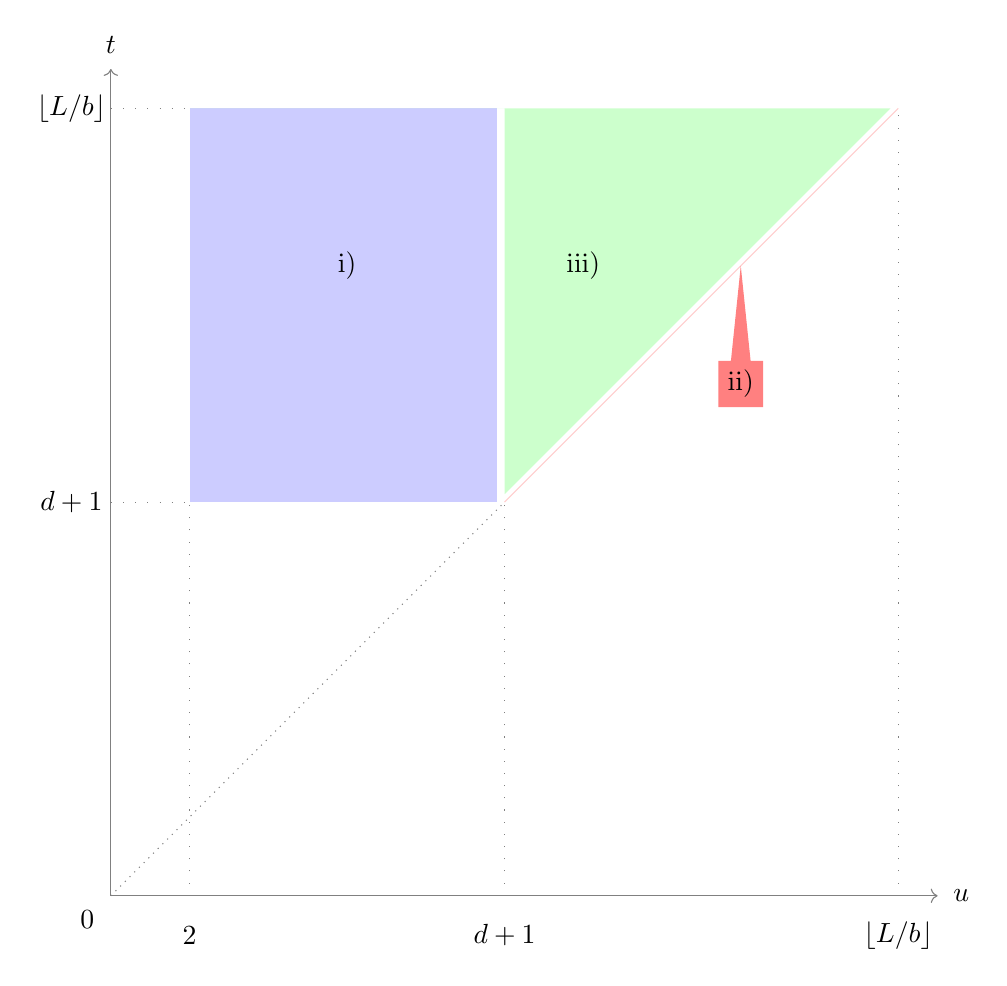
\begin{tikzpicture}[note/.style={rectangle callout, fill=#1}]
	\fill[blue!20] ( 1, 5) -- (4.9, 5) -- (4.9, 10) -- ( 1, 10);
	\fill[green!20] ( 5, 10) -- (5, 5.1) -- (9.9, 10) -- ( 1, 10);
	\draw[red!20] ( 5, 5) -- (10, 10);
	\draw[->,gray] ( 0, 0) -- (10.5, 0);
	\draw[->,gray] ( 0, 0) -- (0, 10.5);
	\draw[gray,loosely dotted] ( 1, 0) -- (1, 5);
	\draw[gray,loosely dotted] ( 10, 0) -- (10, 10);
	\draw[gray,loosely dotted] (  5, 0) -- (5, 5);
	\draw[gray,loosely dotted] (  0, 5) -- ( 1, 5);
	\draw[gray,loosely dotted] (  0,10) -- ( 1,10);
	\draw[gray,dotted] ( 0, 0) -- (5, 5);
	\draw ( -0.3, -0.3) node {$0$} ;
	\draw (10.8, 0) node {$u$} ;
	\draw (0, 10.8) node {$t$} ;
	\draw ( 1, -0.5) node {2} ;
	\draw ( 5, -0.5) node {$d+1$} ;
	\draw (10, -0.5) node {$\lfloor L/b \rfloor$} ;
	\draw ( -0.5, 5) node {$d+1$} ;
	\draw ( -0.5, 10) node {$\lfloor L/b \rfloor$} ;
	\draw ( 3, 8) node {i)} ;
	\draw ( 6, 8) node {iii)} ;
	\node [note=red!50, callout absolute pointer={(8,8)}] at (8,6.5) {ii)};
\end{tikzpicture}

\caption{Parameters $u, t$, where nested summation must be taken}\label{fig:param634}

\end{figure}

$t$-dependency of $F(z, t, u)$ must be considered when $u = t$.
From the above, the parameters domain where summation must be taken can be divided into the following three groups:

\begin{enumerate}[i)]
	%%%%%
	%%%%% i)
	%%%%%
	\item 
	\begin{align}
	\begin{cases}
		2 \leq u < d + 1 & \\
		d + 1 \leq t \leq \lfloor L / b \rfloor & 
	\end{cases}
	\label{eq:zone1_634}
	\end{align}
	%%%%%
	%%%%% ii)
	%%%%%
	\item 
	\begin{align}
	\begin{cases}
		(u, t) = (\tau, \tau) & \\
		d + 1 \leq \tau \leq \lfloor L / b \rfloor & 
	\end{cases}
	\label{eq:zone2_634}
	\end{align}
	%%%%%
	%%%%% iii)
	%%%%%
	\item 
	\begin{align}
	\begin{cases}
		d + 1 \leq u < t & \\
		d + 1 < t \leq \lfloor L / b \rfloor & 
	\end{cases}
	\label{eq:zone3_634}
	\end{align}
\end{enumerate}

For groups i) and iii), the summation with respect to $t$ can be taken first.
By using the relation $\nu = \lfloor L / b \rfloor - d$, Eq.(\ref{eq:rewGin634}) can be rewritten to as follows:
\begin{align}
G(z) =
& \sum_{u = 2}^{d} \log_{2}(u) z^{2} (1-z)^{u-1} \nonumber \\
& + \frac{1}{\nu} \sum_{u = d + 1}^{\lfloor L / b \rfloor} \log_{2}(u) z (1-z)^{u-1} \nonumber \\
& + \frac{1}{\nu} \sum_{u = d + 1}^{\lfloor L / b \rfloor - 1} (\lfloor L / b \rfloor - u) \log_{2}(u) z^{2} (1-z)^{u-1}
\label{eq:rewGin634performance}
\end{align}
With this expression, the computational complexity can be decreased from $\mathcal{O}(\nu^2)$ to $\mathcal{O}(\nu)$.

\subsection{Notes for t-Tuple estimate, LRS estimate, MultiMMC Prediction and LZ78Y prediction estimate}
In the following groups of entropy estimate, we have to handle $t$-tuples (pairs, triples, etc.)
\begin{enumerate}[a)]
	%%%%%
	%%%%% a)
	%%%%%
	\item t-Tuple estimate (NIST SP 800-90B 6.3.5)
	%%%%%
	%%%%% b)
	%%%%%
	\item Longest Repeated Substring (LRS) estimate (NIST SP 800-90B 6.3.6)
	%%%%%
	%%%%% c)
	%%%%%
	\item Multi Most Common in Window Prediction estimate (NIST SP 800-90B 6.3.7)
	%%%%%
	%%%%% d)
	%%%%%
	\item The MultiMMC Prediction estimate (NIST SP 800-90B 6.3.9)
	%%%%%
	%%%%% e)
	%%%%%
	\item The LZ78Y Prediction estimate (NIST SP 800-90B 6.3.10)
\end{enumerate}
In order to express $t$-tuples, bitset or multiprecision integer is used without using array.

\subsection{Notes for Multi Most Common in Window prediction estimate}
In step 3-a-i of 6.3.7 of NIST SP 800-90B, it is required to compute the mode in the previous window of $w_{j}$ before $s_{i}$. 
As the order of $w_{j}$ is 1000, the computational complexity is estimated to be about $\mathcal{O}(1000n)$, and expected to be time-consuming. 
We attempt to reduce time-complexity by preparing histograms of certain lengths in advance, and in step 3-a-i, we use the histograms that fit within the target window, and compute the unavailable parts on-demand basis.

\clearpage
%%%%%%%%%%%%%%%%%%%%%%%%%%%%%%%%%%%%%%%%%%%%%%%%%%%%%%%%%%%%%%%%%%%
%%%%%
%%%%%
%%%%%
%%%%%%%%%%%%%%%%%%%%%%%%%%%%%%%%%%%%%%%%%%%%%%%%%%%%%%%%%%%%%%%%%%%
\section{Additional implementation notes for t-Tuple estimate, LRS estimate using Longest Common Prefix}
%%%%%%%%%%%%%%%%%%%%%%%%%%%%%%%%%%%%%%%%%%%%%%%%%%%%%%%%%%%%%%%%%%%
%%%%%
%%%%%
%%%%%
%%%%%%%%%%%%%%%%%%%%%%%%%%%%%%%%%%%%%%%%%%%%%%%%%%%%%%%%%%%%%%%%%%%
\subsection{An issue of naive implementation for t-Tuple estimate and LRS estimate}
The naive implementation of t-Tuple estimate and LRS estimate consumes huge memory $\approx$ few giga-bytes, to store unique t-Tuple. 
Here, it is stated that Longest Common Prefix can be used for t-Tuple and LRS estimates, and naive algorithm is provided\cite{JoshaHill}.
Note here that \cite{MIT} provides good introduction for Longest Common Prefix and its calculating algorithm.
Next optimized algorithms are provided to perform t-Tuple and LRS estimates\cite{Kaufer}.
However, it is unclear about how to derive the whole algorithms, except for ``Count Aggregation'' (hereafter denoted as ``cascading algorithm'').

So let us consider a more intuitive algorithm to perform t-Tuple and LRS estimates in the following subsection.

%%%%%%%%%%%%%%%%%%%%%%%%%%%%%%%%%%%%%%%%%%%%%%%%%%%%%%%%%%%%%%%%%%%
%%%%%
%%%%%
%%%%%
%%%%%%%%%%%%%%%%%%%%%%%%%%%%%%%%%%%%%%%%%%%%%%%%%%%%%%%%%%%%%%%%%%%
\subsection{Derivation of more intuitive algorithms for t-Tuple estimate and LRS estimate}
Provided that Longest Common Prefix array $(LCP[1], \ldots, LCP[L])$ has been calculated from input $\mib{S}$, 
$LCP[j]$ changes with respect to index $j$, so let us consider the following three cases: 
\begin{enumerate}[a)]
	\item $LCP[j - 1] < LCP[j] \qquad (j \in [2, L])$,
	\item $LCP[j - 1] = LCP[j] \qquad (j \in [2, L])$,
	\item $LCP[j - 1] > LCP[j] \qquad (j \in [2, L])$.
\end{enumerate}

We may call case a) as ``climb up'' case, case b) as ``traverse'' case, and case c) as ``climb down'' case.

For brevity, let us use $\eta_{j}$ to denote $LCP[j]$,  or simply $\eta$ by omitting index $j$.
Let us consider a run length of LCP array at index $j$, and denote $\lambda_{\eta_{j}}$ as the run length.

Normally several minimum and maximum points can be found in LCP array, 
so let us consider the range from one local minimum to the next as a single ``peak'', and introduce an array $\tilde{q}_{\textrm{work}}[\eta]$ representing run length value with respect to the ``height'' $\eta$ (which is equal to a value in LCP array) in currently climbing peak.
Considering that normally there are multiple peaks in LCP array, let us introduce an array $\tilde{q}_{\textrm{master}}[\eta]$ storing the maximum run length for each $\eta$ appeared in the LCP array.

For case a), let us store the previous run length value $\lambda_{\eta_{j-1}}$ to $\tilde{q}_{\textrm{work}}[\eta_{j - 1}]$, and assign new run length value $\lambda_{\eta_{j}}$ as 1.
Note that the part of algorithm is highlighted in \colorbox{hlblue!25}{light blue} in Algorithms \ref{alg:TupleCountMain} and \ref{alg:LRSMain}.

For case b), let us increment $\lambda_{\eta_{j}}$ by 1.
Note that the part of algorithm is highlighted in  \colorbox{Pomme!10}{light green} in Algorithms \ref{alg:TupleCountMain} and \ref{alg:LRSMain}.

For case c), the run lengths of LCP values for $(LCP[j] + 1, \ldots, LCP[j - 1])$ can be determined by Algorithm \ref{alg:Accum}, which is ``cascading algorithm''.
Note that the part of algorithm is highlighted in  \colorbox{Heliotrope!10}{pale purple} in Algorithms \ref{alg:TupleCountMain} and \ref{alg:LRSMain}.

For case c) or ``climb down'' case, update $\tilde{q}_{\textrm{master}}$ to store longer run lengths, and also run lengths for higher $\eta$ values, by comparing $\tilde{q}_{\textrm{work}}$ and $\tilde{q}_{\textrm{master}}$.

Finally the required array $Q[i]$ where $i \in [1, t]$ can be calculated by the following relation:
\begin{align}
Q[i] = \tilde{q}_{\textrm{master}}[i] + 1.
\end{align}

\clearpage
\subsection{Additional implementation notes for t-Tuple estimate using Longest Common Prefix}
%%%%%%%%%%%%%%%%%%%%%%%%%%%%%%%%%%%%%%%%%%%%%%%%%%%%%%%%%%%%%%%%%%%
%%%%%
%%%%%
%%%%%
%%%%%%%%%%%%%%%%%%%%%%%%%%%%%%%%%%%%%%%%%%%%%%%%%%%%%%%%%%%%%%%%%%%

%%%\begin{shadebox}
\begin{algorithm}
%%%\setstretch{1.35}
\setstretch{1.2}
%%%%%
%%%%%
%%%%%
%\begin{minipage}{\hsize}
%%%%%
%%%%%
%%%%%
%\begin{algorithm}
\caption{Rewritten steps 1 and 2 in $t$-Tuple Estimate}\label{alg:TupleCountMain}
%\label{alg:myalgo}
\begin{algorithmic}[1]
%%%%%
%%%%%
%%%%%
\Require input dataset $\mib{S} = (s_{1}, \ldots, S_{L})$ where $s_{i} \in A = \{ x_{1}, \ldots, x_{k}\}$
%Graph $\mathcal{G}$ ($\mathcal{V}$, $\mathcal{E}$); input features $\{x_v, \forall{v} \in \mathcal{V}\}$; depth $K$; weight matrices $W^k, \forall{\mathcal{\textit{k}}} \in \{1, ...,K\}$; non-linearity $\sigma$; differentiable aggregator functions AGGREGATE$_k$, $x_v, \forall{k} \in \{1, ...,K\}$; neighborhood function $\mathcal{N}: v \leftarrow 2^\mathcal{V}$
                \Ensure an integer array of $i$-tuple counts for $i \in \{ 1, 2, \ldots, t\}$
%%%%%
%%%%%
%%%%%
%\setcounter{ALG@line}{1}%
\State Compute the Longest Common Prefix array $LCP[j] (j \in \{ 1, 2, \ldots, L \})$ from $\mib{S}$.
\State $\displaystyle \eta_{\textrm{max}} \gets \textrm{\textbf{max}}_{j \in \{ 1, 2, \ldots, L \}} LCP[j]$
\Statex \Comment {$\eta_{\textrm{max}}$ coincide with $\nu$ in Longest Repeated Substring (LRS) Estimate.}
\For{$\eta \gets 1, \textrm{\textbf{max}}(\eta_{\textrm{max}}, 1)$}
	\State $\tilde{q}_{\textrm{master}}[\eta] \gets 0$
	\State $\tilde{q}_{\textrm{work}}[\eta] \gets 0$
\EndFor

%%%%%\State $\eta_{\textrm{prev}} \gets 0$
%%%%%\State $\eta_{\textrm{current}} \gets 0$
\State $\eta_{\textrm{prev}} \gets LCP[1]$
\State $\lambda \gets 1$
%%%%%
%%%%%\State $\eta_{\textrm{max}} \gets LCP[1]$

\For {$j \gets 2, L$}
	\State $\eta_{\textrm{current}} \gets LCP[j]$
%%%%%
%%%%%\Statex \tikzmk{A}%
%%%%%	\If {$\eta_{\textrm{max}} < LCP[j]$}
%%%%%		\State $\eta_{\textrm{max}} \gets LCP[j]$
%%%%%		\Statex \Comment {update $\eta_{\textrm{max}}$}
%%%%%	\EndIf
%%%%%\tikzmk{B}
%%%%%\boxit{hlblue}
%%%%%
	\If {$\eta_{\textrm{prev}} < \eta_{\textrm{current}}$}
\Statex \tikzmk{A}
		\If {$0 < \eta_{\textrm{prev}}$}
			\State $\tilde{q}_{\textrm{work}}[\eta_{\textrm{prev}}] \gets \lambda$
		\EndIf
		\State $\lambda \gets 1$
\tikzmk{B}
\boxit{hlblue}
	\ElsIf {$\eta_{\textrm{prev}} = \eta_{\textrm{current}}$}
\Statex \tikzmk{A}
		\If {$\eta_{\textrm{current}} = 0$}
			\Statex \Comment {This condition corresponds to consecutive 0-values in array LCP.}
%%%%%			\If {$\tilde{q}_{\textrm{master}}[1] < \lambda$}
%%%%%				\State $\tilde{q}_{\textrm{master}}[1] \gets \lambda$
%%%%%				\Statex \Comment {update 1-tuple count}
%%%%%			\EndIf

			\State $\lambda \gets 1$
			\Statex \Comment {consecutive 0-values in array LCP mean different 1-tuple. }

		\Else
			\State $\lambda \gets \lambda + 1$
		\EndIf
\tikzmk{B}
\boxit{Pomme!40}
	\Else
\Statex \tikzmk{A}
		\State \textbf{AccumulateLambda}($\mib{\tilde{q}}_{\textrm{work}}, \eta_{\textrm{prev}}, \eta_{\textrm{current}}, \lambda$)
%%%%%		\State $\tilde{q}_{\textrm{work}}[\eta_{\textrm{prev}}] \gets \lambda$
%%%%%
%%%%%		\For{$\eta \gets (\eta_{\textrm{prev}} - 1) \Downto \textrm{\textbf{max}}(\eta_{\textrm{current}}, 1) $}
%%%%%			\State $\tilde{q}_{\textrm{work}}[\eta] \gets \tilde{q}_{\textrm{work}}[\eta] + \tilde{q}_{\textrm{work}}[\eta + 1] $
%%%%%			\Statex \Comment {sum up $\lambda$ and update the array $\tilde{q}$}
%%%%%		\EndFor
		
		\State \textbf{UpdateLambda}($\lambda, \mib{\tilde{q}}_{\textrm{work}}, \eta_{\textrm{current}}$)
%%%%%		\If {$\eta_{\textrm{current}} = 0$}
%%%%%			\State $\lambda \gets 1$
%%%%%		\Else
%%%%%			\State $\lambda \gets (\tilde{q}_{\textrm{work}}[\eta_{\textrm{current}}] + 1)$
%%%%%		\EndIf
%%%%%		\If {$\eta_{\textrm{current}} = 0$}
%%%%%		\Else
%%%%%			\State $\tilde{q}_{\textrm{work}}[\eta_{\textrm{current}}] \gets \tilde{q}_{\textrm{work}}[\eta_{\textrm{current}}] + \tilde{q}_{\textrm{work}}[\eta_{\textrm{current}} + 1] $
%%%%%		\EndIf

		\State \textbf{UpdateQTildeMaster}($\mib{\tilde{q}}_{\textrm{master}}, \mib{\tilde{q}}_{\textrm{work}}, \eta_{\textrm{prev}}, \eta_{\textrm{current}}$)
%%%%%		\For{$\eta \gets \eta_{\textrm{prev}} \Downto (\eta_{\textrm{current}} + 1)$}
%%%%%			\If {$\tilde{q}_{\textrm{master}}[\eta] < \tilde{q}_{\textrm{work}}[\eta]$}
%%%%%				\State $\tilde{q}_{\textrm{master}}[\eta] \gets \tilde{q}_{\textrm{work}}[\eta]$
%%%%%				\Statex \Comment {update $\eta$-tuple count}
%%%%%			\EndIf
%%%%%		\EndFor

		\State \textbf{ResetQTildeWork}($\mib{\tilde{q}}_{\textrm{work}}, \eta_{\textrm{prev}}, \eta_{\textrm{current}}$)
%%%%%		\For{$\eta \gets \eta_{\textrm{prev}} \Downto \textrm{\textbf{max}}(\eta_{\textrm{current}}, 1)$}
%%%%%			\State $\tilde{q}_{\textrm{work}}[\eta] \gets 0$
%%%%%			\Statex \Comment {reset to zero for future computation}
%%%%%		\EndFor
\Statex \tikzmk{B}
\boxit{Heliotrope!40}
	\EndIf

	\State $\eta_{\textrm{prev}} \gets \eta_{\textrm{current}}$
\EndFor
%%%%%
%%%%%
%%%%%
\Statex \tikzmk{A}
%%%%%
%%%%%
%%%%%
\State \textbf{AccumulateLambda}($\mib{\tilde{q}}_{\textrm{work}}, \eta_{\textrm{prev}}, 0, \lambda$)
%%%%%
%%%%%
%%%%%
\State \textbf{UpdateQTildeMaster}($\mib{\tilde{q}}_{\textrm{master}}, \mib{\tilde{q}}_{\textrm{work}}, \eta_{\textrm{prev}}, 0$)
%%%%%
%%%%%
%%%%%
\tikzmk{B}
\boxit{Heliotrope!40}
%%%%%
%%%%%
%%%%%
\State $t \gets \textrm{\textbf{max}} \left( \left\{ \eta \in \{1, \dots, \eta_{\textrm{max}}\} \mid \tilde{q}_{\textrm{master}}[\eta] \geq 34 \right\} \right)$
\Statex \Comment {Find the largest $t$ such that the number of occurrences of the most common $t$-tuple in $\mib{S}$ is at least 35. This can be rewritten as shown above using $\mib{\tilde{q}}_{\textrm{master}}$.}
%%%%%
%%%%%
%%%%%
\State return \textbf{CalcQ}($\mib{\tilde{q}}_{\textrm{master}}, t$)
%%%%%
%%%%%
%%%%%
%%%%%\State return Q
\end{algorithmic}
\end{algorithm}
%%%%%
%%%%%
%%%%%
%\end{minipage}
%%%%%
%%%%%
%%%%%
%%%%%\end{shadebox}

\clearpage
%%%%%%%%%%%%%%%%%%%%%%%%%%%%%%%%%%%%%%%%%%%%%%%%%%%%%%%%%%%%%%%%%%%
%%%%%
%%%%%
%%%%%
%%%%%%%%%%%%%%%%%%%%%%%%%%%%%%%%%%%%%%%%%%%%%%%%%%%%%%%%%%%%%%%%%%%
\subsection{Additional implementation notes for LRS estimate using Longest Common Prefix}
\begin{algorithm}
%%%\setstretch{1.35}
\setstretch{1.2}
%%%%%
%%%%%
%%%%%
%\begin{minipage}{\hsize}
%%%%%
%%%%%
%%%%%
%\begin{algorithm}
\caption{Rewritten steps 1, 2 and 3 in Longest Repeated Substring (LRS) Estimate}\label{alg:LRSMain}
%\label{alg:myalgo}
\begin{algorithmic}[1]
%%%%%
%%%%%
%%%%%
\Require input dataset $\mib{S} = (s_{1}, \ldots, S_{L})$ where $s_{i} \in A = \{ x_{1}, \ldots, x_{k}\}$
%Graph $\mathcal{G}$ ($\mathcal{V}$, $\mathcal{E}$); input features $\{x_v, \forall{v} \in \mathcal{V}\}$; depth $K$; weight matrices $W^k, \forall{\mathcal{\textit{k}}} \in \{1, ...,K\}$; non-linearity $\sigma$; differentiable aggregator functions AGGREGATE$_k$, $x_v, \forall{k} \in \{1, ...,K\}$; neighborhood function $\mathcal{N}: v \leftarrow 2^\mathcal{V}$
                \Ensure string $status$, a real value $\hat{p}$
%%%%%
%%%%%
%%%%%
%\setcounter{ALG@line}{1}%
\State Compute the Longest Common Prefix array $LCP[j] (j \in \{ 1, 2, \ldots, L \})$ from $\mib{S}$.
\State $\displaystyle \eta_{\textrm{max}} \gets \textrm{\textbf{max}}_{j \in \{ 1, 2, \ldots, L \}} LCP[j]$
\If {$\eta_{\textrm{max}} < 1$}
	\State return (``$\nu$ not found'', NaN)
	\Statex \Comment {$\nu$ cannot be found, therefore estimate cannot be computed.}
\EndIf
\State $\nu \gets \eta_{\textrm{max}}$
\Statex \Comment {It is ensured that $\nu \ge 1$.}
%\Statex \Comment {$\eta_{\textrm{max}}$ coincide with $\nu$ in Longest Repeated Substring (LRS) Estimate.}
\For{$\eta \gets 1, \nu$}
	\State $\tilde{q}_{\textrm{master}}[\eta] \gets 0$
	\State $\tilde{q}_{\textrm{work}}[\eta] \gets 0$
	\State $\sigma[\eta] \gets 0$
%%%%%	\State $P[\eta] \gets 0$
\EndFor

%%%%%\State $\eta_{\textrm{prev}} \gets 0$
%%%%%\State $\eta_{\textrm{current}} \gets 0$
\State $\eta_{\textrm{prev}} \gets LCP[1]$
\State $\lambda \gets 1$
%%%%%
%%%%%\State $\eta_{\textrm{max}} \gets LCP[1]$

\For {$j \gets 2, L$}
	\State $\eta_{\textrm{current}} \gets LCP[j]$
%%%%%
%%%%%
%%%%%
	\If {$\eta_{\textrm{prev}} < \eta_{\textrm{current}}$}
%%%%%
%%%%%
%%%%%
	\Statex \tikzmk{A}
		\If {$0 < \eta_{\textrm{prev}}$}
			\State $\tilde{q}_{\textrm{work}}[\eta_{\textrm{prev}}] \gets \lambda$
		\EndIf
		\State $\lambda \gets 1$
	\tikzmk{B}
	\boxit{hlblue}
%%%%%
%%%%%
%%%%%
	\ElsIf {$\eta_{\textrm{prev}} = \eta_{\textrm{current}}$}
%%%%%
%%%%%
%%%%%
	\Statex \tikzmk{A}
		\If {$\eta_{\textrm{current}} = 0$}
			\Statex \Comment {This condition corresponds to consecutive 0-values in array LCP.}
%%%%%			\If {$\tilde{q}_{\textrm{master}}[1] < \lambda$}
%%%%%				\State $\tilde{q}_{\textrm{master}}[1] \gets \lambda$
%%%%%				\Statex \Comment {update 1-tuple count}
%%%%%			\EndIf

			\State $\lambda \gets 1$
			\Statex \Comment {consecutive 0-values in array LCP mean different 1-tuple. }
%%%%%
%%%%%
%%%%%
%%%%%				\State $\sigma[1] \gets \sigma[1] + 1$
%%%%%				\Statex \Comment {$C_{i} = 2$, }
%%%%%
%%%%%
%%%%%
		\Else
			\State $\lambda \gets \lambda + 1$
		\EndIf
	\tikzmk{B}
	\boxit{Pomme!40}
%%%%%
%%%%%
%%%%%
	\Else
%%%%%
%%%%%
%%%%%
	\Statex \tikzmk{A}
		\State \textbf{AccumulateLambda}($\mib{\tilde{q}}_{\textrm{work}}, \eta_{\textrm{prev}}, \eta_{\textrm{current}}, \lambda$)
%%%%%
%%%%%
%%%%%
		\State \textbf{UpdateNumerator}($\mib{\sigma}, \mib{\tilde{q}}_{\textrm{work}}, \eta_{\textrm{prev}}, \eta_{\textrm{current}}$)
%%%%%
%%%%%
%%%%%
		\State \textbf{UpdateLambda}($\lambda, \mib{\tilde{q}}_{\textrm{work}}, \eta_{\textrm{current}}$)
%%%%%
%%%%%
%%%%%
		\State \textbf{UpdateQTildeMaster}($\mib{\tilde{q}}_{\textrm{master}}, \mib{\tilde{q}}_{\textrm{work}}, \eta_{\textrm{prev}}, \eta_{\textrm{current}}$)
%%%%%
%%%%%
%%%%%
		\State \textbf{ResetQTildeWork}($\mib{\tilde{q}}_{\textrm{work}}, \eta_{\textrm{prev}}, \eta_{\textrm{current}}$)
%%%%%
%%%%%
%%%%%
	\Statex \tikzmk{B}
	\boxit{Heliotrope!40}
	\EndIf

	\State $\eta_{\textrm{prev}} \gets \eta_{\textrm{current}}$
\EndFor
%%%%%
%%%%%
%%%%%
\Statex \tikzmk{A}
%%%%%
%%%%%
%%%%%
\State \textbf{AccumulateLambda}($\mib{\tilde{q}}_{\textrm{work}}, \eta_{\textrm{prev}}, 0, \lambda$)
%%%%%
%%%%%
%%%%%
\State \textbf{UpdateNumerator}($\mib{\sigma}, \mib{\tilde{q}}_{\textrm{work}}, \eta_{\textrm{prev}}, 0$)
%%%%%
%%%%%
%%%%%
\State \textbf{UpdateQTildeMaster}($\mib{\tilde{q}}_{\textrm{master}}, \mib{\tilde{q}}_{\textrm{work}}, \eta_{\textrm{prev}}, 0$)
%%%%%
%%%%%
%%%%%
\tikzmk{B}
\boxit{Heliotrope!40}
%%%%%
%%%%%
%%%%%
\State $u \gets \textrm{\textbf{min}} \left( \left\{ \eta \in \{1, \dots, \nu\} \mid \tilde{q}_{\textrm{master}}[\eta] < 34 \right\} \right)$
\Statex \Comment {Find the smallest $u$ such that the number of occurrences of the most common $u$-tuple in $\mib{S}$ is less than 35. This can be rewritten as shown above using $\mib{\tilde{q}}_{\textrm{master}}$.}
%%%%%
%%%%%
%%%%%
\State $\hat{p} \gets $ \textbf{CalcPHat}($\mib{\sigma}, u, \nu$)
%%%%%\State $\displaystyle \hat{p} \gets \textrm{\textbf{max}} \left( \left( P[u] \right)^{\frac{1}{u}}, \ldots, \left( P[\nu] \right)^{\frac{1}{\nu}} \right) $
\Statex \Comment {Compute the estimated average collision probability per string symbol as $P_{\textrm{max},W} = \left( P_{W}\right)^{\frac{1}{W}}$.  Let $\hat{p} = \textrm{max}\left( P_{\textrm{max},u}, \ldots, P_{\textrm{max},\nu}\right)$.}
\State return (``Success'', $\hat{p}$)
%%%%%
%%%%%
%%%%%
%%%%%\State return Q
\end{algorithmic}
\end{algorithm}
%%%%%
%%%%%
%%%%%
%\end{minipage}
%%%%%
%%%%%
%%%%%
%%%%%\end{shadebox}

\clearpage
%%%%%%%%%%%%%%%%%%%%%%%%%%%%%%%%%%%%%%%%%%%%%%%%%%%%%%%%%%%%%%%%%%%
%%%%%
%%%%%
%%%%%
%%%%%%%%%%%%%%%%%%%%%%%%%%%%%%%%%%%%%%%%%%%%%%%%%%%%%%%%%%%%%%%%%%%
\subsection{Auxiliary routines}
%%%%%%%%%%%%%%%%%%%%%%%%%%%%%%%%%%%%%%%%%%%%%%%%%%%%%%%%%%%%%%%%%%%
%%%%%
%%%%% algorithms applicable for t-tuple estimate and LRS estimate
%%%%%
%%%%%%%%%%%%%%%%%%%%%%%%%%%%%%%%%%%%%%%%%%%%%%%%%%%%%%%%%%%%%%%%%%%
\begin{algorithm}
  \caption{AccumulateLambda}\label{alg:Accum}
  \begin{algorithmic}[1]
    \Procedure{AccumulateLambda}{$\mib{\tilde{q}}_{\textrm{work}}, \eta_{\textrm{prev}}, \eta_{\textrm{current}}, \lambda$}
		\State $\tilde{q}_{\textrm{work}}[\eta_{\textrm{prev}}] \gets \lambda$

		\For{$\eta \gets (\eta_{\textrm{prev}} - 1) \Downto \textrm{\textbf{max}}(\eta_{\textrm{current}}, 1) $}
			\State $\tilde{q}_{\textrm{work}}[\eta] \gets \tilde{q}_{\textrm{work}}[\eta] + \tilde{q}_{\textrm{work}}[\eta + 1] $
			\Statex \Comment {sum up $\lambda$ and update the array $\tilde{q}$}
		\EndFor


    \EndProcedure
  \end{algorithmic}
\end{algorithm}

\begin{algorithm}
  \caption{UpdateLambda}\label{alg:UpdateLambda}
  \begin{algorithmic}[1]
    \Procedure{UpdateLambda}{$\lambda, \mib{\tilde{q}}_{\textrm{work}}, \eta_{\textrm{current}}$}
		\If {$\eta_{\textrm{current}} = 0$}
			\State $\lambda \gets 1$
		\Else
			\State $\lambda \gets (\tilde{q}_{\textrm{work}}[\eta_{\textrm{current}}] + 1)$
		\EndIf
    \EndProcedure
  \end{algorithmic}
\end{algorithm}

\begin{algorithm}
  \caption{UpdateQTildeMaster}\label{alg:UpdateQTildeMaster}
  \begin{algorithmic}[1]
    \Procedure{UpdateQTildeMaster}{$\mib{\tilde{q}}_{\textrm{master}}, \mib{\tilde{q}}_{\textrm{work}}, \eta_{\textrm{prev}}, \eta_{\textrm{current}}$}
		\For{$\eta \gets \eta_{\textrm{prev}} \Downto (\eta_{\textrm{current}} + 1)$}
			\If {$\tilde{q}_{\textrm{master}}[\eta] < \tilde{q}_{\textrm{work}}[\eta]$}
				\State $\tilde{q}_{\textrm{master}}[\eta] \gets \tilde{q}_{\textrm{work}}[\eta]$
				\Statex \Comment {update $\eta$-tuple count}
			\EndIf
		\EndFor
    \EndProcedure
  \end{algorithmic}
\end{algorithm}

\begin{algorithm}
  \caption{ResetQTildeWork}\label{alg:ResetTheta}
  \begin{algorithmic}[1]
    \Procedure{ResetQTildeWork}{$\mib{\tilde{q}}_{\textrm{work}}, \eta_{\textrm{prev}}, \eta_{\textrm{current}}$}
		\For{$\eta \gets \eta_{\textrm{prev}} \Downto \textrm{\textbf{max}}(\eta_{\textrm{current}}, 1)$}
			\State $\tilde{q}_{\textrm{work}}[\eta] \gets 0$
			\Statex \Comment {reset to zero for future computation}
		\EndFor
    \EndProcedure
  \end{algorithmic}
\end{algorithm}

%%%%%%%%%%%%%%%%%%%%%%%%%%%%%%%%%%%%%%%%%%%%%%%%%%%%%%%%%%%%%%%%%%%
%%%%%
%%%%% algorithm applicable only for t-tuple estimate
%%%%%
%%%%%%%%%%%%%%%%%%%%%%%%%%%%%%%%%%%%%%%%%%%%%%%%%%%%%%%%%%%%%%%%%%%
\begin{algorithm}
  \caption{CalcQ}\label{alg:CalcQ}
  \begin{algorithmic}[1]
    \Function{CalcQ}{$\mib{\tilde{q}}_{\textrm{master}}, t$}
%%%%%		\For{$\eta \gets 1, (t + 1)$}
%%%%%			\State $Q[\eta] \gets 0$
%%%%%		\EndFor
		\For{$\eta \gets 1, t$}
			\State $Q[\eta] \gets \tilde{q}_{\textrm{master}}[\eta] + 1$
		\EndFor

		\State return $\mib{Q} = ( Q[1], \ldots, Q[t])$
    \EndFunction
  \end{algorithmic}
\end{algorithm}

%%%%%%%%%%%%%%%%%%%%%%%%%%%%%%%%%%%%%%%%%%%%%%%%%%%%%%%%%%%%%%%%%%%
%%%%%
%%%%% algorithm applicable only for LRS estimate
%%%%%
%%%%%%%%%%%%%%%%%%%%%%%%%%%%%%%%%%%%%%%%%%%%%%%%%%%%%%%%%%%%%%%%%%%
\begin{algorithm}
  \caption{UpdateNumerator}\label{alg:UpdateNumerator}
  \begin{algorithmic}[1]
    \Procedure{UpdateNumerator}{$\mib{\sigma}, \mib{\tilde{q}}_{\textrm{work}}, \eta_{\textrm{prev}}, \eta_{\textrm{current}}$}
		\For{$\eta \gets \eta_{\textrm{prev}} \Downto (\eta_{\textrm{current}} + 1) $}
			\Statex \Comment {Here, $\tilde{q}_{\textrm{work}}[\eta_{\textrm{current}}]$ is a snapshot at a given point in time, therefore, updating $\sigma[\eta]$ where $\eta > \eta_{\textrm{current}}$ makes sense.}
			\If {$\tilde{q}_{\textrm{work}}[\eta] + 1 \ge 2$}
				\State $\displaystyle \sigma[\eta] \gets \sigma[\eta] + \binom{\tilde{q}_{\textrm{work}}[\eta] + 1}{2}$
			\EndIf
		\EndFor

    \EndProcedure
  \end{algorithmic}
\end{algorithm}

%%%%%%%%%%%%%%%%%%%%%%%%%%%%%%%%%%%%%%%%%%%%%%%%%%%%%%%%%%%%%%%%%%%
%%%%%
%%%%% algorithm applicable only for LRS estimate
%%%%%
%%%%%%%%%%%%%%%%%%%%%%%%%%%%%%%%%%%%%%%%%%%%%%%%%%%%%%%%%%%%%%%%%%%
\begin{algorithm}
  \caption{CalcPHat}\label{alg:CalcPHat}
  \begin{algorithmic}[1]
    \Function{CalcPHat}{$\mib{\sigma}, u, \nu$}
%%%%%		\For{$\eta \gets 1, (t + 1)$}
%%%%%			\State $Q[\eta] \gets 0$
%%%%%		\EndFor
		\For{$W \gets u, \nu$}
			\State $\displaystyle P[W] \gets \frac{ \sigma[W] }{ \binom{L - W + 1}{2} }$
		\EndFor
		\State $\displaystyle \hat{p} \gets \textrm{\textbf{max}} \left( \left( P[u] \right)^{\frac{1}{u}}, \ldots, \left( P[\nu] \right)^{\frac{1}{\nu}} \right) $
		\State return $\hat{p}$
%%%%%		\State return $\mib{P} = ( P[u], \ldots, P[\nu] ) $
    \EndFunction
  \end{algorithmic}
\end{algorithm}


\clearpage
%%%%%%%%%%%%%%%%%%%%%%%%%%%%%%%%%%%%%%%%%%%%%%%%%%%%%%%%%%%%%%%%%%%%%%%%%%%%%%%
%%%%%
%%%%% Bibliography
%%%%%
%%%%%%%%%%%%%%%%%%%%%%%%%%%%%%%%%%%%%%%%%%%%%%%%%%%%%%%%%%%%%%%%%%%%%%%%%%%%%%%
\setcounter{section}{3}
\begin{thebibliography}{99}
\addcontentsline{toc}{section}{References}
% 1
\bibitem{SP80090B}
Meltem S\"{o}nmez Turan,
Elaine Barker,
John Kelsey,
Kerry A. McKay,
Mary L. Baish,
Mike Boyle
\textit{Recommendation for the Entropy Sources Used for Random Bit Generation},
NIST Special Publication 800-90B, Jan. 2018
% 2
\bibitem{AIS31draft2022}
M. Peter and W. Schindler,
\textit{A Proposal for Functionality Classes for Random Number Generators}
Version 2.35 - DRAFT,
September 2, 2022.
\url{https://www.bsi.bund.de/SharedDocs/Downloads/EN/BSI/Certification/Interpretations/AIS_31_Functionality_classes_for_random_number_generators_e.pdf?__blob=publicationFile&v=7}
% 3
\bibitem{MathHandbook}
Franck W. J. Oliver,
Daniel W. Lozier,
Ronald F. Boisvert,
Charles W. Clark,
\textit{NIST Handbook of Mathematical Functions},
National Institute of Standards and Technology, 2010
% 6
\bibitem{CorrectionsSP80090B}
G. Sakurai, \textit{Proposed list of corrections for NIST SP 800-90B 6.3 Estimators}, Dec. 2022
\url{https://github.com/g-g-sakura/AnotherEntropyEstimationTool/blob/main/documentation/ProposedListOfCorrections_SP800-90B.pdf}
% 7
\bibitem{JoshaHill}
Joshua E. Hill, \textit{Algorithms for t-tuple and LRS Estimates}, June 11, 2018
\url{https://www.untruth.org/~josh/sp80090b/NIST.SP.800-90B%20implementation%20comments%2020191219.pdf}
% 8
\bibitem{MIT}
Thomas H. Cormen, Charles E. Leiserson, Ronald L. Rivest and Clifford Stein, \textit{Introduction to Algorithms (fourth edition)}, The MIT Press.
\url{https://mitpress.mit.edu/9780262046305/introduction-to-algorithms/}

% 9
\bibitem{Kaufer}
Aaron Kaufer, \textit{Further Improvements for SP 800-90B Tuple Counts}, April 10, 2019
\url{https://www.untruth.org/~josh/sp80090b/Kaufer%20Further%20Improvements%20for%20SP%20800-90B%20Tuple%20Counts.pdf}
\end{thebibliography}

\end{document}
